
\section{Simulations}\label{sec-sim}

We next turn to the test methods from Section \ref{sec-test-equality}. The simulation design extends the setup from above. We generate data from the model $Y_{it} = m_i(\frac{t}{T}) + \varepsilon_{it}$, where the number of time series $i$ is set to $n = 15$ and we consider different time series lengths $T$. For each $i$, the errors $\varepsilon_{it}$ are drawn from the AR(1) model $\varepsilon_{it} = a \varepsilon_{i,t-1} + \eta_{it}$, where as before $a = 0.267$ and the innovations $\eta_{it}$ are i.i.d.\ normally distributed with mean $0$ and variance $0.35$. To generate data under the null $H_0: m_1 = \ldots = m_n$, we let $m_i = 0$ for all $i$ without loss of generality. To produce data under the alternative, we define $m_1(u) = \beta \, (u - 0.5) $ with $\beta = 0.75, 1, 1.25$ and set $m_i = 0$ for all $i \ne 1$. Hence, all trend functions are the same except for $m_1$ which is an increasing linear function. We here use a linear function rather than a broken line as the normalization constraint $\int_0^1 m_1(u) du = 0$ is directly satisfied in this case. 

\addtocounter{table}{-1} 
\begin{table}[t]
\footnotesize{
\begin{center}
\caption{Size of the multiscale test from Section \ref{sec-test-equality} for $n=15$ time series, different sample sizes $T$ and nominal sizes $\alpha$.}
\label{tab:size_equality}
\renewcommand{\arraystretch}{1.2}
% latex table generated in R 3.4.3 by xtable 1.8-2 package
% 
\begin{tabular}{cccc}
  \hline
  & \multicolumn{3}{c}{nominal size $\alpha$} \\
 $T$ & 0.01 & 0.05 & 0.1 \\
 \hline
250 & 0.096 & 0.096 & 0.096 \\ 
  300 & 0.096 & 0.096 & 0.096 \\ 
  500 & 0.096 & 0.096 & 0.096 \\ 
  1000 & 0.096 & 0.096 & 0.096 \\ 
   \hline
\end{tabular}

\end{center}}
\footnotesize{
\begin{center}
\caption{Power of the multiscale test from Section \ref{sec-test-equality} for $n=15$ time series, different sample sizes $T$ and nominal sizes $\alpha$. Each panel corresponds to a different slope parameter $\beta$.}\label{tab:power_equality}
\begin{subtable}[b]{0.32\textwidth}
\centering
\caption{$\beta = 0.75$}\label{tab:power_75_equality}
\renewcommand{\arraystretch}{1.2}
% latex table generated in R 3.4.3 by xtable 1.8-2 package
% 
\begin{tabular}{cccc}
  \hline
  & \multicolumn{3}{c}{nominal size $\alpha$} \\
 $T$ & 0.01 & 0.05 & 0.1 \\
 \hline
250 & 0.354 & 0.557 & 0.687 \\ 
  300 & 0.349 & 0.659 & 0.772 \\ 
  500 & 0.859 & 0.946 & 0.964 \\ 
  1000 & 0.997 & 1.000 & 1.000 \\ 
   \hline
\end{tabular}

\end{subtable}
\begin{subtable}[b]{0.32\textwidth}
\centering
\caption{$\beta = 1.00$}\label{tab:power_100_equality}
\renewcommand{\arraystretch}{1.2}
% latex table generated in R 3.4.3 by xtable 1.8-2 package
% 
\begin{tabular}{cccc}
  \hline
  & \multicolumn{3}{c}{nominal size $\alpha$} \\
 $T$ & 0.01 & 0.05 & 0.1 \\
 \hline
250 & 0.758 & 0.895 & 0.946 \\ 
350 & 0.902 & 0.976 & 0.986 \\ 
  500 & 0.997 & 0.999 & 0.999 \\ 
  1000 & 1.000 & 1.000 & 1.000 \\ 
   \hline
\end{tabular}

\end{subtable}
\begin{subtable}[b]{0.32\textwidth}
\centering
\caption{$\beta = 1.25$}\label{tab:power_125_equality}
\renewcommand{\arraystretch}{1.2}
% latex table generated in R 3.4.3 by xtable 1.8-2 package
% 
\begin{tabular}{cccc}
  \hline
  & \multicolumn{3}{c}{nominal size $\alpha$} \\
 $T$ & 0.01 & 0.05 & 0.1 \\
 \hline
250 & 0.961 & 0.990 & 0.997 \\ 
  300 & 0.991 & 1.000 & 1.000 \\ 
  500 & 1.000 & 1.000 & 1.000 \\ 
  1000 & 1.000 & 1.000 & 1.000 \\ 
   \hline
\end{tabular}

\end{subtable}
\end{center}}
\vspace{-0.4cm}
\end{table}

The test is implemented analogously as before. We in particular use an Epanechnikov kernel, we define the grid $\mathcal{G}_T$ as in \eqref{grid-sim-app} and we set the two tuning parameters $L_1$ and $L_2$ to $\lfloor \sqrt{T} \rfloor$ and $\lfloor 2\sqrt{T} \rfloor$, respectively. In order to compute the critical values of the test, we simulate $1000$ values of the statistic $\Phi_{n,T}$ defined in Section \ref{subsec-test-equality-test} and compute their empirical $(1-\alpha)$ quantile $q_{n,T}(\alpha)$. Note that the statistic $\Phi_{n,T}$ depends on the estimators $\widehat{\sigma}_i^2$ of the long-run error variances $\sigma_i^2$. This implies that for each simulated sample, we have to recompute the empirical quantile $q_{n,T}(\alpha)$ and thus the critical value of the test. This is of course computationally extremely expensive. In order to circumvent this issue, we make the additional assumption that the long-run error variance is known to be the same across $i$, that is, $\sigma_i^2 = \sigma^2$ for all $i$. Under this assumption, we can estimate $\sigma^2$ by $\widehat{\sigma}^2 = (\sum_{i = 1}^n\widehat{\sigma_i}^2)/n$, and the Gaussian statistic $\Phi_{n,T}$ simplifies to $\Phi_{n,T} = \max_{1 \le i < j \le n} \Phi_{ij,T}$ with $\Phi_{ij,T} = \max_{(u,h) \in \mathcal{G}_T} \{ | \phi_{ij,T}(u,h)| - \lambda(h) \}$ and $\phi_{ij,T}(u,h) = \sum_{t=1}^T w_{t,T}(u,h) \{ (Z_{it} - \bar{Z}_i) - (Z_{jt} - \bar{Z}_j)\}$. This statistic does not depend on the estimators $\widehat{\sigma}_i^2$ anymore. We thus do not need to recompute the critical values for each simulated sample, which decreases the running time significantly.


The simulation results are reported in Tables \ref{tab:size_equality} and \ref{tab:power_equality}. The entries of the tables are computed in the same way as those in Tables \ref{tab:size_shape} and \ref{tab:power_shape}. Inspecting Table \ref{tab:size_equality}, the actual size of the test can be seen to approximate the nominal target $\alpha$ quite well even for small values of $T$. Moreover, as can be seen from Table \ref{tab:power_equality}, the test also has reasonable power against the alternatives considered. For the smallest slope $\beta=0.75$ and the smallest sample size $T = 250$, the power is only moderate, reflecting the fact that the alternative is not very far away from the null. However, as we increase the slope $\beta$ and the sample size $T$, the power quickly increases. 
%For the largest slope $\beta = 1.25$ and $T=350$, we already reach a power of $1.00$.


We finally investigate the finite sample performance of the clustering algorithm from Section \ref{subsec-test-equality-clustering}. To do so, we partition the $n = 15$ time series into $N=3$ groups, each containing $5$ time series. Specifically, we set $G_1 = \{1,\ldots,5\}$, $G_2 = \{6,\ldots,10\}$ and $G_3 =  \{11,\ldots,15\}$. Moreover, we define the group-specific trend functions $g_1$, $g_2$ and $g_3$ by $g_1(u) = 0$, $g_2(u) = 1 \cdot (u - 0.5)$ and $g_3(u) =  (- 1) \cdot (u - 0.5)$. In order to compute our estimators of the groups $G_1$, $G_2$, $G_3$ and their number $N = 3$, we use the same implementation as before followed by the clustering procedure from Section \ref{subsec-test-equality-clustering}. The estimation results are reported in Table \ref{tab:clustering_results}. The entries in Table $\ref{tab:clustering_number_of_groups}$ are computed as the number of simulations for which $\widehat{N} = N$ divided by the total number of simulations. They thus specify the empirical probabilities with which the estimate $\widehat{N}$ is equal to the true number of groups $N = 3$. Analogously, the entries of Table $\ref{tab:clustering_groups}$ give the empirical probabilities with which the estimated group structure $\{ \widehat{G}_1,\ldots,\widehat{G}_{\widehat{N}}\}$ equals the true one $\{G_1,G_2,G_3\}$. 


\addtocounter{table}{-1} 
\begin{table}[t]
\footnotesize{
\begin{center}
\caption{Clustering results for different sample sizes $T$ and nominal sizes $\alpha$.}\label{tab:clustering_results}
\begin{subtable}[b]{0.48\textwidth}
\centering
\caption{Empirical probabilities that \\ $\widehat{N} = N$}\label{tab:clustering_number_of_groups}
\renewcommand{\arraystretch}{1.2}
% latex table generated in R 3.4.3 by xtable 1.8-2 package
% 
\begin{tabular}{cccc}
  \hline
  & \multicolumn{3}{c}{nominal size $\alpha$} \\
 $T$ & 0.01 & 0.05 & 0.1 \\
 \hline
250 & 0.500 & 1.000 & 1.000 \\ 
   \hline
\end{tabular}

\end{subtable}
\begin{subtable}[b]{0.48\textwidth}
\centering
\caption{\centering Empirical probabilities that $\{ \widehat{G}_1,\ldots,\widehat{G}_{\widehat{N}}\} = \{ G_1,G_2,G_3\}$}\label{tab:clustering_groups}
\renewcommand{\arraystretch}{1.2}
% latex table generated in R 3.4.3 by xtable 1.8-2 package
% 
\begin{tabular}{cccc}
  \hline
  & \multicolumn{3}{c}{nominal size $\alpha$} \\
 $T$ & 0.01 & 0.05 & 0.1 \\
 \hline
250 & 0.581 & 0.747 & 0.776 \\ 
  300 & 0.741 & 0.886 & 0.889 \\ 
  500 & 0.984 & 0.974 & 0.966 \\ 
  1000 & 0.998 & 0.987 & 0.972 \\ 
   \hline
\end{tabular}

\end{subtable}
\end{center}}
\vspace{-0.5cm}
\end{table}


The simulation results nicely illustrate the theoretical properties of our clustering algorithm. According to Proposition \ref{prop-clustering-1}, the probability that $\widehat{N} = N$ and $\{ \widehat{G}_1,\ldots,\widehat{G}_{\widehat{N}}\} = \{G_1,G_2,G_3\}$ should be at least $(1-\alpha)$ asymptotically. For the sample sizes $T = 500$ and $T = 1000$, the empirical probabilities reported in Table \ref{tab:clustering_results} can indeed be seen to exceed the value $(1-\alpha)$ as predicted by Proposition \ref{prop-clustering-1}. Only for $T = 500$ and $\alpha = 0.01$, the empirical probability is slightly below $(1-\alpha)$. For the smaller sample sizes $T=250$ and $T=350$, in contrast, some of the empirical probabilities are much smaller than $(1-\alpha)$. This reflects the asymptotic nature of Proposition \ref{prop-clustering-1} and is not very suprising. It simply mirrors the fact that for small sample sizes, the effective noise level in the simulated data is quite high. Even though some of the empirical probabilities for $T=250$ and $T=350$ are clearly below the target $(1-\alpha)$, they are still quite substantial. Hence, even for these small sample sizes, our estimates $\widehat{N}$ and $\{ \widehat{G}_1,\ldots,\widehat{G}_{\widehat{N}} \}$ are equal to the true values in a large number of simulations. 

\section{Applications}\label{sec-data}
\subsection{Analysis of UK weather station data}\label{subsec-data-2} 


\begin{figure}[t]
\centering
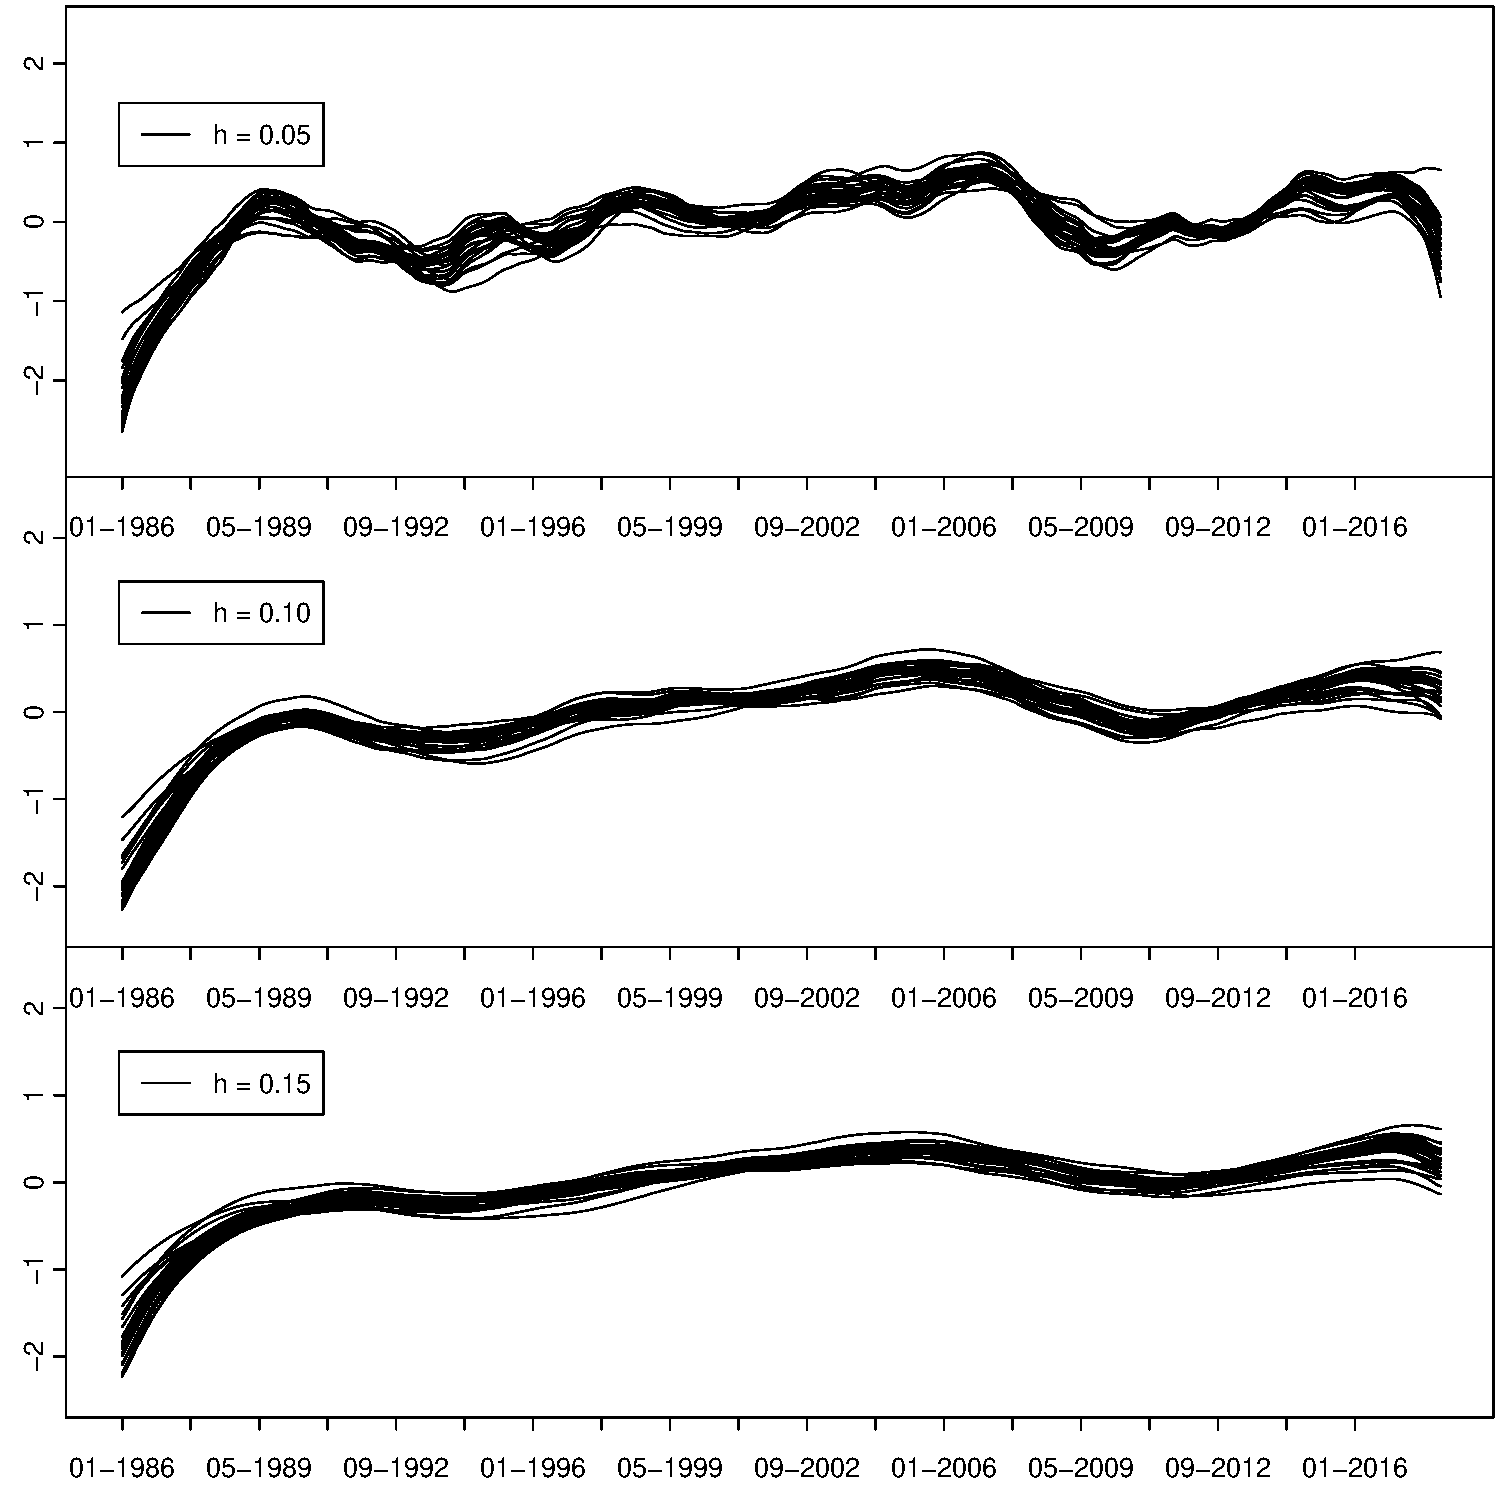
\includegraphics[width=0.8\textwidth]{Plots/stations_data.pdf}
\vspace{0.2cm}
\caption{Local linear kernel estimates of the $n=25$ time trends from the application of Section \ref{subsec-data-2}. Each panel shows the estimates for a different bandwidth $h$.}\label{plot-results-app2}
\end{figure}


To illustrate our test method from Section \ref{sec-test-equality}, we examine a dataset of monthly mean temperatures from $34$ different UK weather stations. The data are publicly available on the webpage of the UK Met Office. We use a subset of $25$ stations for which data are available over the time span from $1986$ to $2017$. We thus observe a time series $\mathcal{Y}_i = \{Y_{it}: 1 \le t \le T \}$ of length $T = 386$ for each station $i \in \{1,\ldots,25\}$. The time series $\mathcal{Y}_i$ is assumed to follow the model 
\begin{equation}\label{model2-app}
Y_{it} = \alpha_i(t) + m_i\Big(\frac{t}{T}\Big) + \varepsilon_{it}, 
\end{equation}
where $m_i$ is an unknown nonparametric time trend and $\alpha_i(t)$ is a month-specific intercept which captures the seasonality pattern in the data. We suppose that $\alpha_i(t) = \alpha_i(t + 12 \ell)$ for any integer $\ell$, that is, we have a different intercept $\alpha_i(k)$ for each month $k = 1,\ldots,12$. The test method and the underlying theory from Section \ref{sec-test-equality} can be easily adapted to model \eqref{model2-app}, which is a slight extension of model \eqref{model2}. The details are provided below. As in Section \ref{subsec-data-1}, the error process $\mathcal{E}_i = \{ \varepsilon_{it}: 1 \le t \le T \}$ is assumed to have the AR(1) structure $\varepsilon_{it} = a_i \varepsilon_{i,t-1} + \eta_{it}$ for each $i$, where $\eta_{it}$ are i.i.d.\ innovations with mean zero.  


We aim to test whether the time trend $m_i$ is the same at each of the $25$ weather stations. In other words, we want to test the null hypothesis $H_0: m_1 = \ldots = m_n$ with $n = 25$ in model \eqref{model2-app}. To do so, we apply the multiscale test from Section \ref{sec-test-equality} with two minor modifications: (i) We define $\widehat{Y}_{it} = Y_{it} - \widehat{\alpha}_i(t)$, where $\widehat{\alpha}_i(t)$ is an estimator of $\alpha_i(t)$. In particular, we set $\widehat{\alpha}_i(t) = \widehat{\alpha}_i(k)$ for any $t = k + 12 \ell$ with $1 \le k \le 12$ and some $\ell \in \integers$, where $\widehat{\alpha}_i(k) = T_k^{-1} \sum_{t = 1}^T \ind_k(t) Y_{it}$ with $\ind_k(t) = \ind(t = k + \lfloor (t-1)/12 \rfloor \cdot 12)$ and $T_k = \sum_{t=1}^T \ind_k(t)$ for $1 \le k \le 12$. (ii) We define the Gaussian statistic $\Phi_{n,T}$ as in Section \ref{subsec-test-equality-test} with $\phi_{ij,T}(u,h) = \sum_{t=1}^T w_{t,T}(u,h) \{ \widehat{\sigma}_i (Z_{it} - \bar{Z}_i(t)) - \widehat{\sigma}_j (Z_{jt} - \bar{Z}_j(t))\}$, where $\bar{Z}_i(t) = \sum_{k=1}^{12} 1_k(t) \{ T_k^{-1} \sum_{s = 1}^T \ind_k(s) Z_{is} \}$. Apart from these two modifications, the multiscale test is constructed exactly as described in Section \ref{sec-test-equality}. We implement the test in the same way as in the simulations of Section \ref{sec-sim}. 


We are now ready to apply the test procedure to the data. Figure \ref{plot-results-app2} depicts local linear estimates of the trend functions $m_i$ for the $n=25$ different stations. Each panel corresponds to a different bandwidth $h$. As can be seen, for a given bandwidth $h$, the fits look very similar to each other. Visual inspection thus suggests that there are no strong differences between the time trends $m_i$. Our test confirms this impression. It does not reject the null hypothesis at the most common levels $\alpha = 0.01, 0.05, 0.1$. Hence, the test does not provide any evidence for a violation of the null. 

